\subsection{Определение частных производных и их геометрический смысл} \label{sec:2.1}

\begin{tbox}{Функция одной переменной}
	Рассмотрим функцию \( y = f(x) \), где \( x \in E \subset \mathbb{R} \) и \( y \in E \).
	Запишем определение производной в точке \( x_0 \). Для этого зададим приращение аргумента \( \Delta x = x - x_0 \) (или \( x = x_0 + \Delta x \)) и вычислим приращение функции:
	\[
	\Delta f(x_0) = f(x_0 + \Delta x) - f(x_0).
	\]

	Производной функции в точке называется предел отношения приращения функции к приращению аргумента при \( \Delta x \to 0 \):
	\begin{align}
		\lim_{\Delta x \to 0} \frac{\Delta f(x_0)}{\Delta x} = f'(x_0) = \frac{dy}{dx}\bigg|_{x = x_0} = \frac{df(x_0)}{dx}.
		\label{eq:15}
	\end{align}
\end{tbox}

\begin{tbox}{Функция многих переменных}
	Теперь обобщим определение (\ref{eq:15}) на случай функции многих переменных \( y = f(\vec{x}) = f(x_1, x_2, \dots, x_k) \). Поскольку дифференцирование проводится по одной переменной, зададим приращение в точке \( \vec{x}_0 \) только по переменной \( x_i \). Вектор приращений имеет вид:
	\[
	\Delta \vec{x} = (0, \dots, 0, \Delta x_i, 0, \dots, 0),
	\]

	тогда:
	\[
	\vec{x} = \vec{x}_0 + \Delta \vec{x} = \left(x_0^{(1)}, \dots, x_0^{(i-1)}, x_0^{(i)} + \Delta x_i, x_0^{(i+1)}, \dots, x_0^{(k)}\right).
	\]

	Соответствующее частное приращение функции:
	\begin{align}
		\Delta_i f(\vec{x}_0) = f\left(x_{0_1}, \dots, x_{0_{i-1}}, x_{0_i} + \Delta x_i, x_{0_{i+1}}, \dots, x_{0_k}\right) - f\left(x_{0_1}, \dots, x_{0_k}\right).
		\label{eq:16}
	\end{align}
\end{tbox}

\begin{tbox}{Частная производная}
	По аналогии с \cref{eq:15} определим частную производную как предел:
	\begin{align}
		\exists \lim_{\Delta x_i \to 0} \frac{\Delta_i f(\vec{x}_0)}{\Delta x_i}.
		\label{eq:17}
	\end{align}

	Если этот предел существует, то он называется частной производной функции \( y = f(\vec{x}) \) в точке \( \vec{x}_0 \) по переменной \( x_i \) и обозначается:
	\begin{align}
		f_{x_i}^{\prime}(\vec{x}_0) = \frac{\partial f(\vec{x}_0)}{\partial x_i}.
		\label{eq:18}
	\end{align}
	\textbf{Замечание}: Запись \( \frac{df(\vec{x}_0)}{dx_i} \) не используется для частных производных.
\end{tbox}

\begin{tbox}{Частные производные первого порядка}
	Поскольку производная вычисляется по одной из \( k \) независимых переменных, функция \( y = f(x_1, x_2, \dots, x_k) \) имеет \( k \) частных производных первого порядка:
	\begin{align}
		\frac{\partial f}{\partial x_1}, \frac{\partial f}{\partial x_2}, \dots, \frac{\partial f}{\partial x_k}.
		\label{eq:19}
	\end{align}
\end{tbox}

\begin{tbox}{Функция двух переменных}
	Рассмотрим частный случай \( z = f(x, y) \). В точке \( M_0(x_0, y_0) \) зададим приращение \( \Delta x \) по переменной \( x \). Частное приращение:
	\begin{align}
		\Delta_x z(M_0) = f(x_0 + \Delta x, y_0) - f(x_0, y_0).
		\label{eq:20}
	\end{align}

	Частная производная по \( x \):
	\begin{align}
		\frac{\partial z(M_0)}{\partial x} = \lim_{\Delta x \to 0} \frac{\Delta_x z(M_0)}{\Delta x}.
		\label{eq:21}
	\end{align}

	Аналогично для приращения \( \Delta y \) по \( y \):
	\begin{align}
		\frac{\partial z(M_0)}{\partial y} = \lim_{\Delta y \to 0} \frac{f(x_0, y_0 + \Delta y) - f(x_0, y_0)}{\Delta y}.
		\label{eq:22}
	\end{align}
\end{tbox}

\begin{tbox*}{Правила вычисления}
	При вычислении \( \frac{\partial z}{\partial x} \) переменная \( y \) считается константой, и наоборот. Используются стандартные правила дифференцирования:
	\begin{itemize}
		\item Производная константы равна нулю.
		\item Константа выносится за знак производной.
	\end{itemize}
\end{tbox*}

\begin{tbox}{Геометрический смысл}
	Функция \( z = f(x, y) \) задаёт поверхность в \( \mathbb{R}^3 \). Точке \( M_0(x_0, y_0) \) соответствует точка \( N(x_0, y_0, z_0) \) на поверхности.\\

	\textbf{Производная по x (\Cref{fig:2.1.1.1})}. При \( y = y_0 \) получаем сечение поверхности плоскостью, параллельной \( XOZ \). Частная производная \( \frac{\partial z}{\partial x} \) равна тангенсу угла \( \alpha \) наклона касательной к этому сечению:
	\[
	\tg \alpha = \frac{\partial z(M_0)}{\partial x}.
	\]

	\textbf{Производная по y (\Cref{fig:2.1.1.2})}. Аналогично, при \( x = x_0 \):
	\[
	\tg \beta = \frac{\partial z(M_0)}{\partial y}.
	\]
\end{tbox}

\begin{figure}[H]
	\centering
	\begin{minipage}{0.45\linewidth}
		\centering
		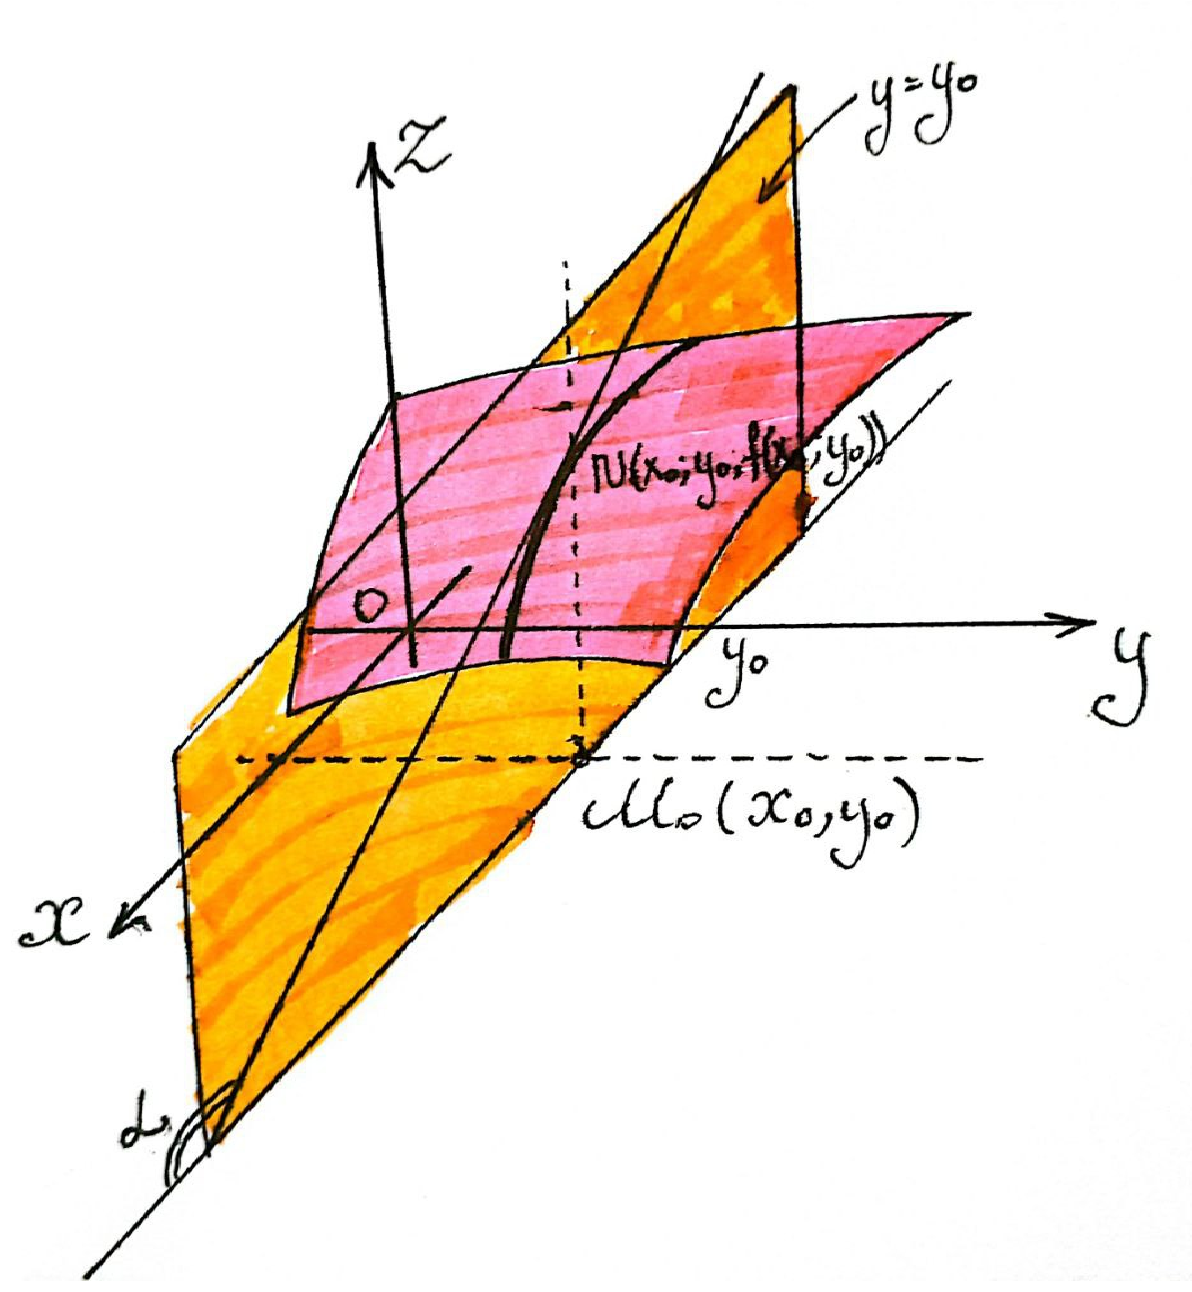
\includegraphics[width=0.9\linewidth]{screenshot011}
		\caption{Геометрический смысл \( \frac{\partial z}{\partial x} \).}
		\label{fig:2.1.1.1}
	\end{minipage}
	\begin{minipage}{0.45\linewidth}
		\centering
		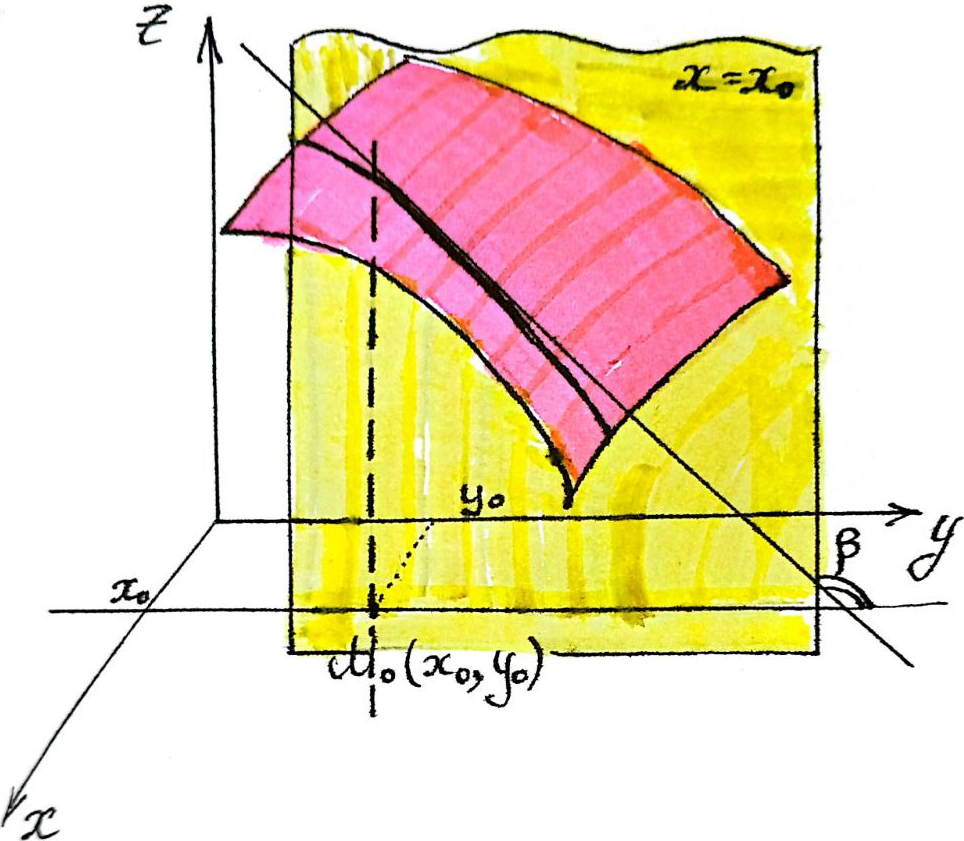
\includegraphics[width=0.9\linewidth]{screenshot012}
		\caption{Геометрический смысл \( \frac{\partial z}{\partial y} \).}
		\label{fig:2.1.1.2}
	\end{minipage}
\end{figure}